\chapter{Installation of the software}
%-------------------------------

\diva is a software designed to run with any operating system (Microsoft Windows, Linux, Mac OS X). The main steps for the the installation are described in this chapter. A more detailed and up-to-date list of instructions is available on the Installation web page of \diva: \url{http://modb.oce.ulg.ac.be/mediawiki/index.php/Diva_installation}

%%while the Graphical User Interface (GUI) is presented in Section~\ref{sec:guiinstall}. Note that the GUI is not up-to-date.

\minitoc

%\newpage



\section{Requirements}
%---------------------

The basic requirements to compile and run \diva are:
\begin{enumerate}
\item A command-line interface. With Linux or Mac, the interface is directly available: it is the shell or terminal. With Windows, it is necessary to install a Unix-like environment such as Cygwin (\url{http://www.cygwin.com/}).
\item A Fortran 95 compiler with preprocessing -cpp possibilities, such as:
\begin{itemize}
\item gfortran (\url{http://gcc.gnu.org/wiki/GFortran}),
\item ifort (Intel\textsuperscript{\textregistered}, \url{http://software.intel.com/en-us/intel-compilers}),
\item pgf (Portland Group, \url{http://www.pgroup.com/}).
\end{itemize}    
\item The NetCDF library (\url{http://www.unidata.ucar.edu/software/netcdf/}) for Fortran. Note that the library is available in recent versions of the cygwin installer, but does not properly work in all cases (and you must add the library \texttt{nclib=/usr/lib/libnetcdff.dll.a} into the compiling options). When trying to make the cygwin NetCDF library to work, you might need to use 

\begin{lstlisting}[style=Bash]
[charles@gher13 ~]$ cygcheck netcdfoutput.a
\end{lstlisting}
%$
to see which libraries are still missing (in our case \texttt{sasl}) and therefore to install them with the cygwin installer.  
\end{enumerate}

For a quick visualization of the results, a software able to read and display the content of a NetCDF \index{NetCDF} file is recommended:
\begin{itemize}
\item ncBrowse (\url{http://www.epic.noaa.gov/java/ncBrowse/}, a Java application,
\item Ncview (\url{http://meteora.ucsd.edu/~pierce/ncview_home_page.html}), a visual browser, 
\item Panoply (\url{http://www.giss.nasa.gov/tools/panoply/}, the NASA data viewer for various data formats.
\end{itemize}


\section{Download and extraction of the archive}
%-----------------------------------------
\index{Download}
Select a directory on your local disk (here we install in a directory \directory{\textasciitilde/Software/}) where you want install \diva and download the archive available at \url{http://modb.oce.ulg.ac.be/mediawiki/index.php/DIVA#How_to_get_the_code.3F}.

\begin{lstlisting}[style=Bash]
[charles@gher13 ~]$ cd Software/
[charles@gher13 Software]$ wget http://modb.oce.ulg.ac.be/mediawiki/upload/DIVA/releases/GODIVA_mm_yyyy.tar.gz
\end{lstlisting}

Extract the archive and go in the main directory:
\begin{lstlisting}[style=Bash]
[charles@gher13 Software]$ tar -xvf GODIVA_07_2012.tar.gz
[charles@gher13 Software]$ cd GODIVA_07_2012/
\end{lstlisting}

The directory tree has the following structure: %\newpage 
\begin{lstlisting}[style=Bash]
[charles@gher13 GODIVA_07_2012]$ tree -d -L 2
.
|-- DIVA3D
|   |-- bin
|   |-- divastripped
|   `-- src
|-- Doc
`-- JRA4
    `-- Climatology

7 directories
\end{lstlisting}


\begin{itemize}
\item \directory{DIVA3D/bin/} contains the executables generated by the code compilation. Pre-compiled executables for various operating systems are provided in the sub-folders.
\item \directory{DIVA3D/divastripped/} is the main working directory at the 2-D level. 
\item \directory{DIVA3D/src/} contains the Fortran source code. This is where the compilation has to be done.
\item[]
\item \directory{Doc/} contains the link to publications. For \LaTeX users: you find the corresponding \BibTeX  entries in the file \file{DivaPublications.bib}.
\item \directory{JRA4/Climatology/} is the main working directory at the 3-D and 4-D levels.
\end{itemize}

%----------------------------------------------
\section{Generation of the binaries (executables)}
%----------------------------------------------

There are two possibilities to obtain the binaries: 
\begin{enumerate}
\item Compile the source code.
\item Copy the provided binaries.
\end{enumerate}
The second option is provided for cases where the compilation was not possible, mainly because of missing libraries (e.g., NetCDF) or Fortran compilers.

\subsection{Compilation\label{sec:compilation}}
%-----------------------------------------------

\index{Compilation}
Go in the source directory 
\begin{lstlisting}[style=Bash]
[charles@gher13 GODIVA_07_2012]$ cd DIVA3D/src/Fortran/
\end{lstlisting}
and edit the configuration file \file{divacompile\_options} for the compilation  according to your machine. 

\begin{verbatim}
# Name of the fortran compiler (ex: ifort,gfortran,pgi,...)
compiler=ifort
# Compilation flags
flags='-O3'
# Netcdf library
nclib=/usr/local/lib/netcdf3ifort/libnetcdf.a
...
\end{verbatim}

If your installation knows the \command{nf-config} or \command{nc-config} command, the compiler and the options for the NetCDF \index{NetCDF} library will be detected automatically during the compilation. If you want to check before compilation, type:
\begin{lstlisting}[style=Bash]
[charles@gher13 ~]$ nf-config --fc
gfortran
[charles@gher13 ~]$ nf-config --flibs
-L/usr/lib -lnetcdff -lnetcdf
\end{lstlisting}
Check the options of this command by typing \command{nf-config}, or visit the web page: \url{http://www.unidata.ucar.edu/software/netcdf/workshops/2011/utilities/Nc-config.html}. If you have installed several versions of the NetCDF libraries, you might find several \command{nf-config} on your system, and each of them may provide you different outputs for the two previous commands. In older versions of NetCDF libraries \command{nc-config} was used instead of \command{nf-config}.





Then run the compilation script: 
\begin{lstlisting}[style=Bash]
[charles@gher13 Fortran] divacompileall
\end{lstlisting}
and check the content of the log file (\file{compilation.log}). You should obtain something similar to that:
\begin{verbatim}
Compilation time:  Thu Oct 25 14:21:54 CEST 2012
compiler:          ifort
compilation flags: -O3
Calc directory:       1/1   program compiled
Extensions directory: 12/12 programs compiled
Mesh directory:       9/9   programs compiled
NC directory:         3/3   programs compiled
PlPlot directory:     1/1   programs compiled
Util directory:       38/38 programs compiled
Pipetest directory:   1/1   program compiled
Stabil directory:     28/28 programs compiled
----------------------------------------------------------
TOTAL:                93/93 programs compiled
----------------------------------------------------------
Binaries are located in directory:
/home/charles/Software/GODIVA_07_2012/DIVA3D/bin
\end{verbatim}

\subsection{Direct copy of pre-compiled binaries}

If the compilation failed, go in the \directory{GODIVA\_mm\_yyyy/DIVA3D/bin/} directory and copy directly the binaries available in the sub-directories. For example for Windows with the Cygwin tool:
\begin{lstlisting}[style=Bash]
[charles@gher13 bin] cp -f cygwin/* .
\end{lstlisting}

\section{Run tests\label{sec:divatest}}
%------------------

In the main working directory (\directory{GODIVA\_mm\_yyyy/DIVA3D/divastripped}), run one the two available tests: \command{divatest} and \command{divabigtest}. 


\subsection{Basic test}


\command{divatest} creates basic input files (see Chapter~\ref{chap:general} for details), performs a simple \diva execution, checks if \command{awk} is appropriate and checks if the pipes are supported in your operating system (O.S.). If \command{divatest} hangs during the pipe test, it means pipes are not supported (as for some gfortran versions) and you can use a \command{CTRL-C} to exit. The analysis output can be checked using any software for reading NetCDF\index{NetCDF} files. In this case we use ncview (see Chapter~\ref{chap:postprocessing} for details and installation). 

\begin{lstlisting}[style=Bash]
[charles@gher13 divastripped]$ divatest
...
[charles@gher13 divastripped]$ ncview output/ghertonetcdf/results.nc
\end{lstlisting}
The results you obtain have to be similar to those of Fig.~\ref{fig:diva_test_results}.

\begin{figure}[H]
\centering 
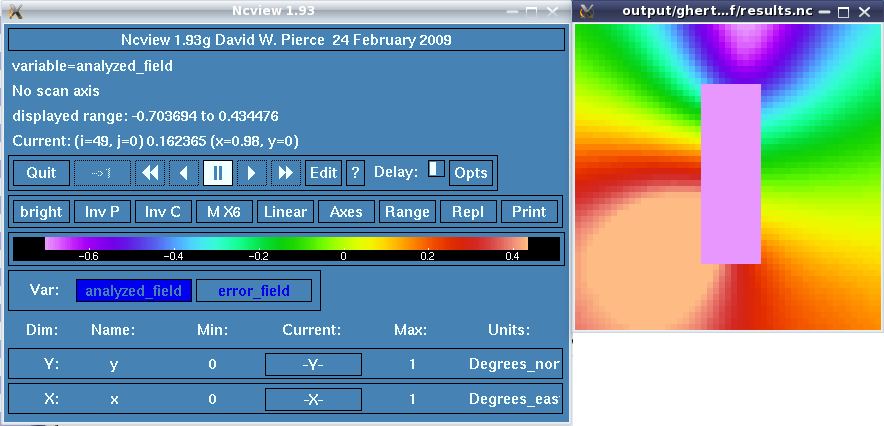
\includegraphics[width=.7\textwidth]{diva_test_results}
\caption{Results obtained with \command{divatest}.\label{fig:diva_test_results}}
\end{figure}


\subsection{Another basic test}

\command{divatest0} creates basic input files for a fine mesh and a single data point in the center of the domain and runs the analysis. You should obtain the Bessel function with a maximum value of 0.5.


\subsection{Large-memory test}
%-----------------------------

\command{divabigtest} creates input files to simulate a case with a large number of data and a very fine mesh. Again, the results, obtained after a few minutes, are viewable using the command:
\begin{lstlisting}[style=Bash]
[charles@gher13 divastripped] ncview output/ghertonetcdf/results.nc
\end{lstlisting}
and should be close to Fig.~\ref{fig:diva_bigtest_results}.

\begin{figure}[H]
\centering 
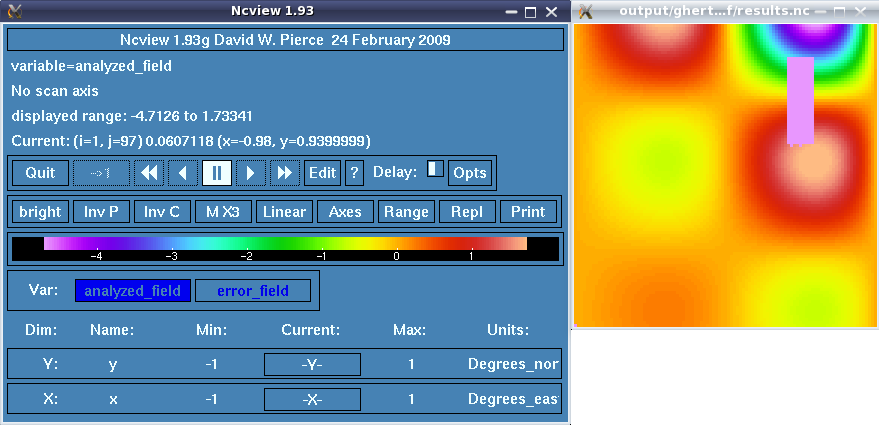
\includegraphics[width=.7\textwidth]{diva_bigtest_results}
\caption{Results obtained with \command{divabigtest}.\label{fig:diva_bigtest_results}}
\end{figure}



%\section{Command Line version}
%%-----------------------------
%
%This version is directly usable through a shell in the \texttt{divastripped} directory. 
%
%\begin{figure}[htpb]
%\centering
%\parbox{.65\textwidth}{
%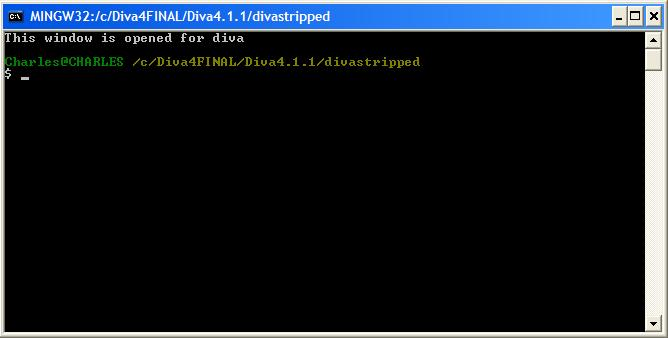
\includegraphics[width=.6\textwidth]{shell}
%}\parbox{.35\textwidth}{
%\caption{\texttt{Msys} shell.\label{shell}}
%}
%\end{figure}
%
%
%\subsection{Windows\label{windowsmsys}}
%%--------------------------------------
%
%You have two possibilities to have a Linux-like shell in your Windows environment:
%
%\begin{enumerate}
%
%\item \texttt{Cygwin}: it can easily be installed (or updated) from \url{http://www.cygwin.com/} by running \texttt{setup.exe} found there. \texttt{Cygwin} is a complete Linux-like environment, thus is recommended to Linux users.
%
%\item \texttt{Msys}: it constitutes the minimal environment under Windows. Its installation is described in the following. 
%
%\end{enumerate}
%
%\subsubsection{\texttt{Msys} installation}
%%-----------------------------------------
%
%If you need to install \texttt{Msys} on your computer:
%\begin{enumerate}
%\item Download the compressed file from\\ 
%\url{http://www.mingw.org/download.shtml}
%%\url{http://prdownloads.sourceforge.net/tcl/msys_mingw8.zip}
%\item Unzip \texttt{msys\_mingw8.zip} (or any recent version) in the chosen directory (let us assume in \texttt{C:/}).
%\item Open the \texttt{msys} shell (Fig. \ref{shell}) by double-clicking on the \texttt{msys} icon (MS-DOS command file) located in the \texttt{msys} folder.
%\end{enumerate}
%

%

%
%\section[Installation checking]{Installation checking \expert}
%%-----------------------------------------
%
%This part is quite technical and is not essential for further use of the software. In directory \texttt{diva-\divaversion/install/} you find a series of tools allowing you to perform an elaborated check of your installation by comparing results of \diva executions with your installation with reference outputs. 
%
%Additional information can be found in \texttt{diva-\divaversion/install/README}.
%
%
%\subsection{\texttt{divamakecheck}}
%%----------------------------------
%
%Apply analysis on test cases listed in \texttt{divachecklist} and compare the results with references by applying \texttt{divacomp}.
%The command\\
%\texttt{divamakecheck -generate}\\
%will create new reference fields for later comparisons. Only developers shall use the \texttt{-generate} option.
%
%\subsection{\texttt{divacomp}}
%%-----------------------------
%
%Compare \texttt{ascii} output files generated by a \diva run with reference files provided with the distribution. Results of the comparison are written in \texttt{check.log}.
%
%
%\subsection{\texttt{divados2unix}}
%%---------------------------------
%
%Apply the conversion from dos-like to unix-like line endings on every \diva\texttt{ascii} file and set the permissions of the executables (\texttt{*.a} files) to 755. 
%
%

